% 
% Annual Cognitive Science Conference
% Sample LaTeX Paper -- Proceedings Format
% 

% Original : Ashwin Ram (ashwin@cc.gatech.edu)       04/01/1994
% Modified : Johanna Moore (jmoore@cs.pitt.edu)      03/17/1995
% Modified : David Noelle (noelle@ucsd.edu)          03/15/1996
% Modified : Pat Langley (langley@cs.stanford.edu)   01/26/1997
% Latex2e corrections by Ramin Charles Nakisa        01/28/1997 
% Modified : Tina Eliassi-Rad (eliassi@cs.wisc.edu)  01/31/1998
% Modified : Trisha Yannuzzi (trisha@ircs.upenn.edu) 12/28/1999 (in process)
% Modified : Mary Ellen Foster (M.E.Foster@ed.ac.uk) 12/11/2000
% Modified : Ken Forbus                              01/23/2004
% Modified : Eli M. Silk (esilk@pitt.edu)            05/24/2005
% Modified : Niels Taatgen (taatgen@cmu.edu)         10/24/2006
% Modified : David Noelle (dnoelle@ucmerced.edu)     11/19/2014
% Modified : Roger Levy (rplevy@mit.edu)     12/31/2018



%% Change "letterpaper" in the following line to "a4paper" if you must.

\documentclass[10pt,letterpaper]{article}
\usepackage{cogsci}
\usepackage{dsfont}
\usepackage{bm}
\usepackage{amssymb}
\usepackage{indentfirst}
\usepackage{graphicx}
\usepackage{subfig}
\usepackage{multirow}

%\cogscifinalcopy % Uncomment this line for the final submission 


\usepackage{pslatex}
\usepackage{apacite}
\usepackage{float} % Roger Levy added this and changed figure/table
                   % placement to [H] for conformity to Word template,
                   % though floating tables and figures to top is
                   % still generally recommended!

%\usepackage[none]{hyphenat} % Sometimes it can be useful to turn off
%hyphenation for purposes such as spell checking of the resulting
%PDF.  Uncomment this block to turn off hyphenation.


%\setlength\titlebox{4.5cm}
% You can expand the titlebox if you need extra space
% to show all the authors. Please do not make the titlebox
% smaller than 4.5cm (the original size).
%%If you do, we reserve the right to require you to change it back in
%%the camera-ready version, which could interfere with the timely
%%appearance of your paper in the Proceedings.



\title{Actual Causes as Changes of State in Continuous Time}
 
\author{{\large \bf Morton Ann Gernsbacher (MAG@Macc.Wisc.Edu)} \\
  Department of Psychology, 1202 W. Johnson Street \\
  Madison, WI 53706 USA
  \AND {\large \bf Sharon J.~Derry (SDJ@Macc.Wisc.Edu)} \\
  Department of Educational Psychology, 1025 W. Johnson Street \\
  Madison, WI 53706 USA}


\begin{document}

\maketitle


\begin{abstract}

\textbf{Keywords:} 
\end{abstract}


\section{Introduction}

Identifying the causes of an event involves not only logical rules but also different senses of ``causation'' that people might have. Let's imagine that, to mitigate false alarms rate and improve the detection of fires, Lilly decides to install at home a dual alarm system that goes off if and only if two chains of ionization and photoelectric detectors are triggered (Fig.\ref{fig:1}a). Lilly wants to test her new system by exposing the detectors to some smoke. At some point a ionization detector starts beeping first while measuring a change in the electrical conductivity of air. It activates the next detector in the sequence which then activates the last one (Fig.\ref{fig:1}b). At this stage Lilly notices that the alarm remains silent. After a while a photoelectric detector starts beeping as well while measuring a change in the transparency of air. It activates the next detector in the sequence which then activates the last one and right after the alarm goes off (Fig.\ref{fig:1}c). 

\begin{figure}[h]
\begin{center}
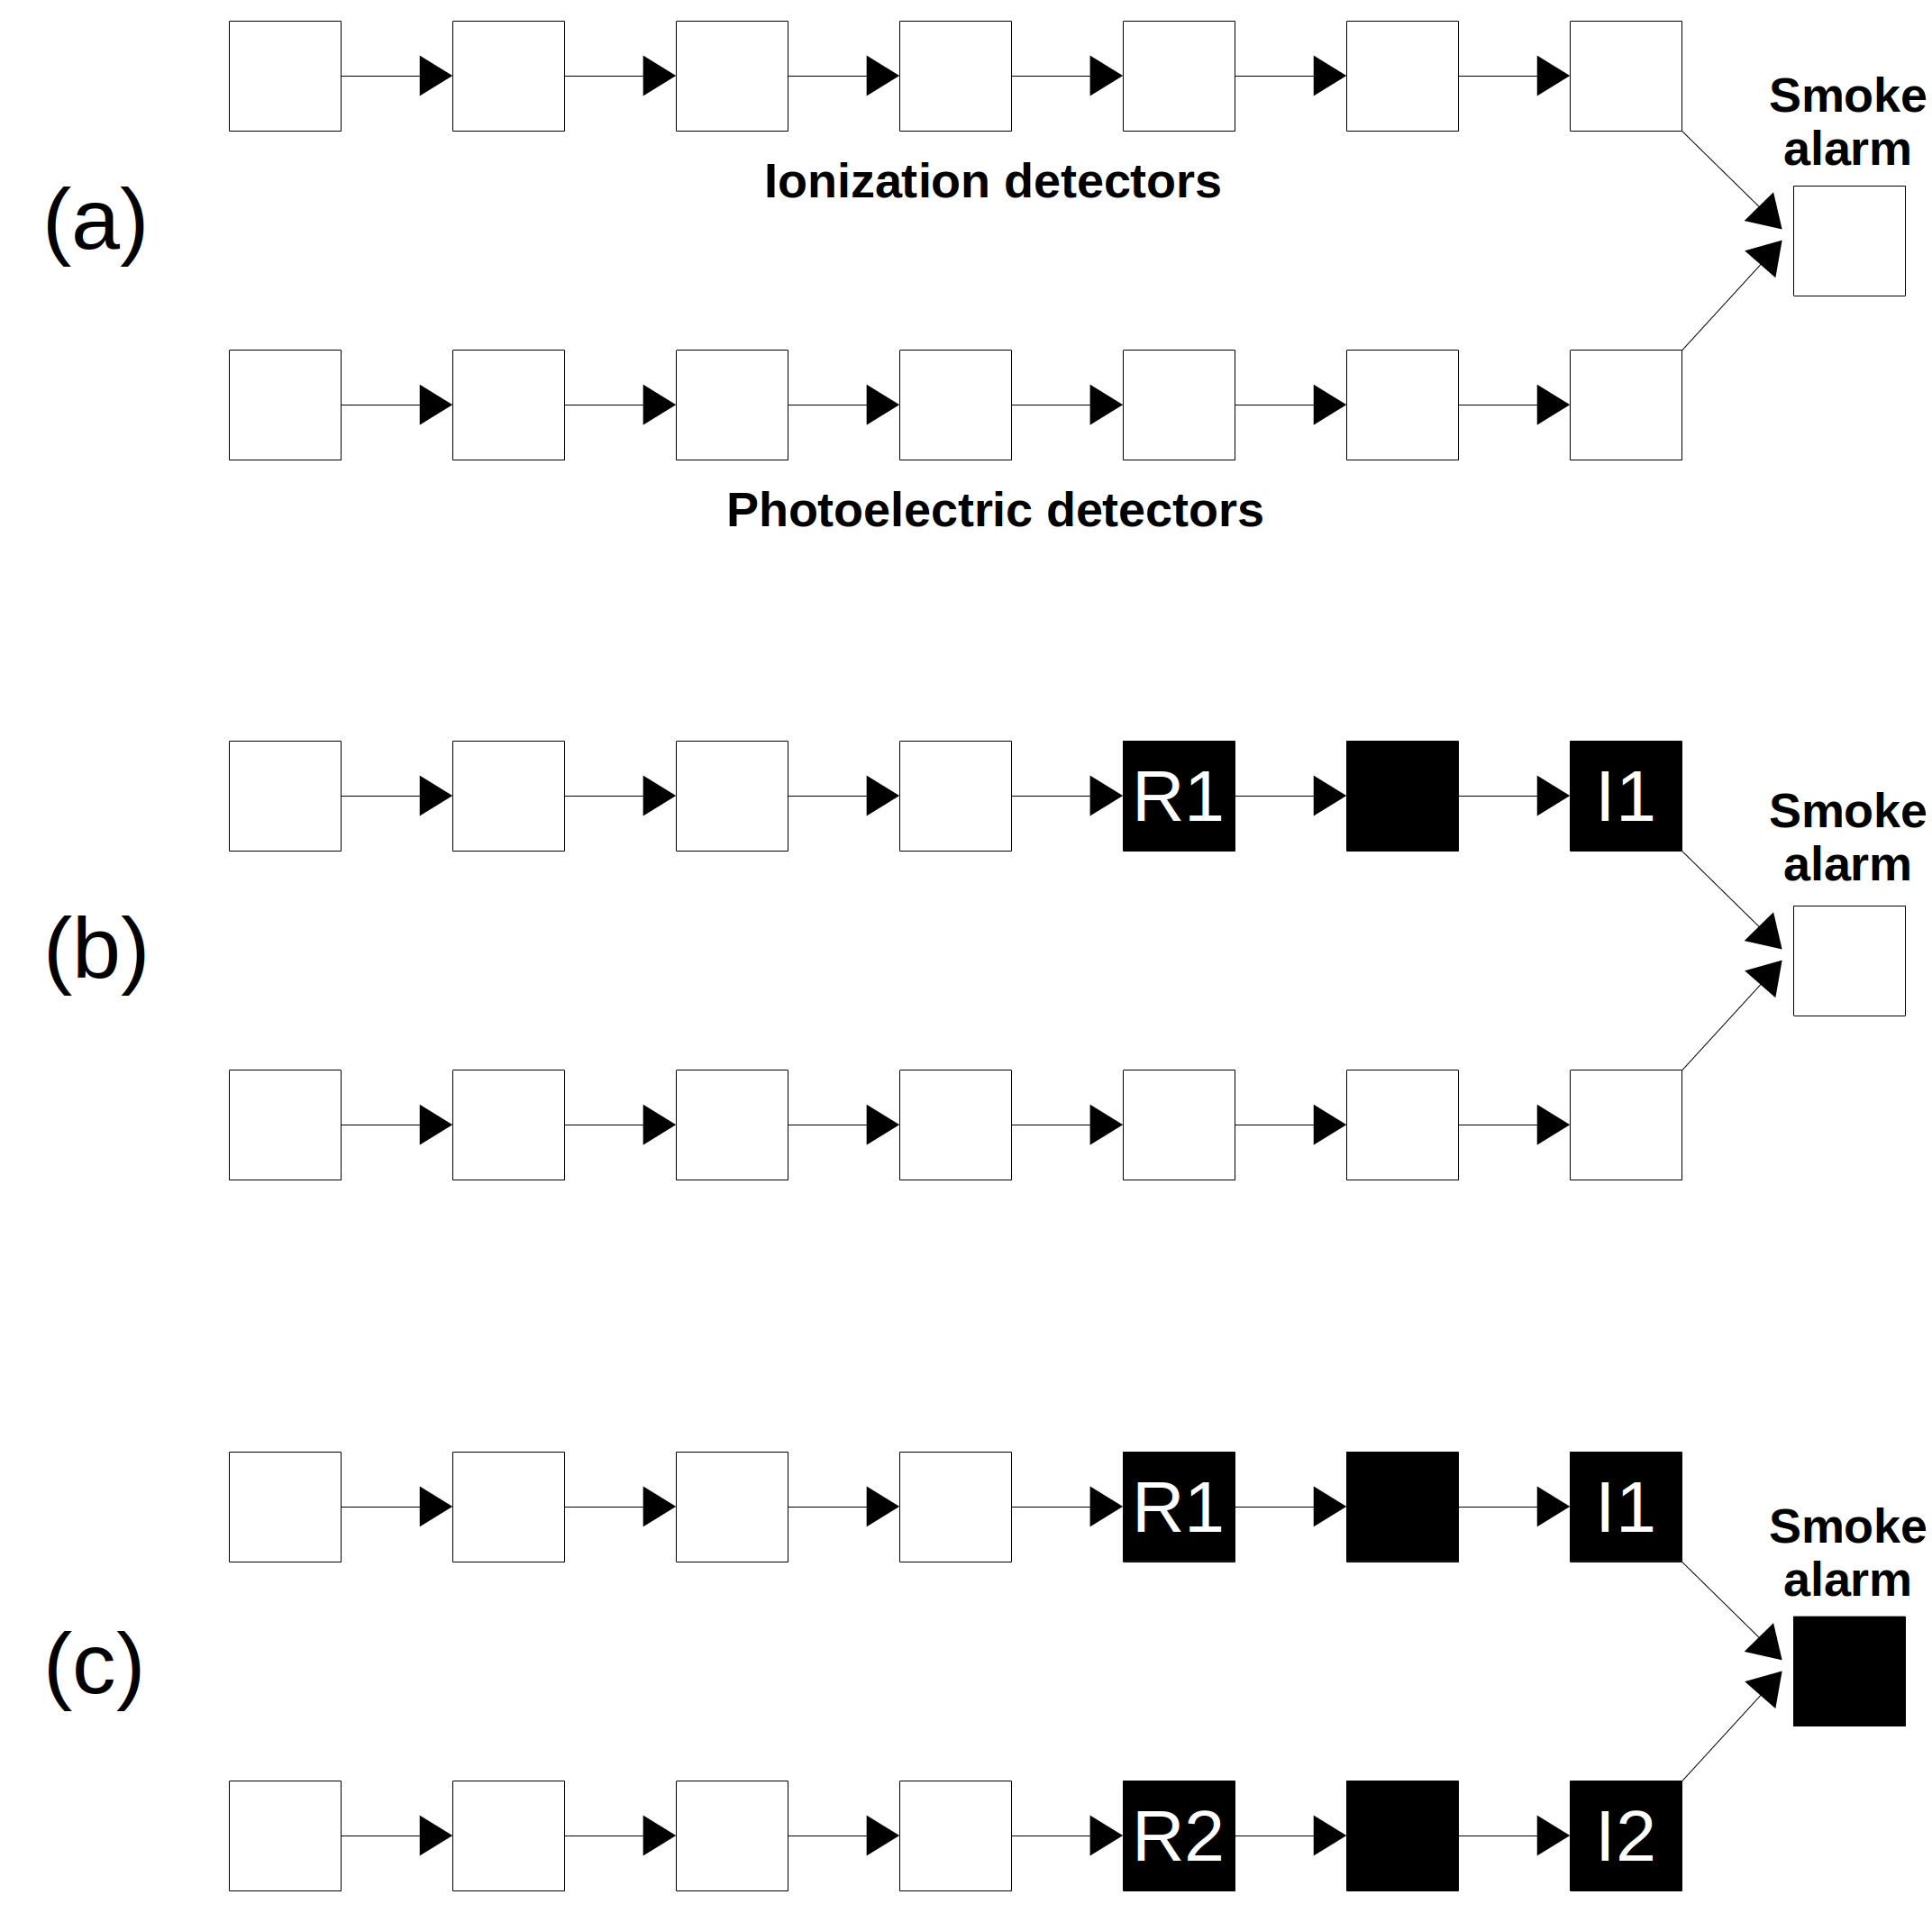
\includegraphics[width=7cm]{intro}
\end{center}
\caption{An example of an AND-Gate causal system. In an AND-Gate for an effect to occur it needs the occurence of all the causes it is linked to. Here for the smoke alarm to go off, both the ionization and photoelectric detectors it is connected to have to be activated. In this scenario the detectors activation spreads over the top chain first (b) and then over the bottom chain leading to the alarm activation (c).} 
\label{fig:1}
\end{figure}

What would Lilly think caused the alarm to go off? Several answers can be considered. Based on logical dependencies, people's causal judgements can state that both the furthest activated ionization detector (first root change ``R1'') and the furthest activated photoelectric detector (second root change ``R2'') are equally the causes of the alarm activation. However a more intuitive answer would be that the provided temporal information influences people's choice toward one cause more than the other one. An important selection criterium could be how recent a candidate cause is compared to another one and would lead for instance to the following preferences: R2 $\succ$ R1, and I2 $\succ$ I1 (``I2'' and ``I1'' being respectively the second and first immediate changes). Nonetheless we can imagine other cases where people potentially rely in part on another type of temporal criterium: let's imagine that the activation of the ionization detectors starts before and finishes after the activation of the photoelectric detectors, such that R1 and I2 are linked by a \textit{continuous sequence of changes}. In that case this is the activation of the oldest root change R1 and not the most recent root change R2 that initiate a continuous sequence of changes until the activation of the alarm. In such situations we want to know what people would consider as the main cause of the system.

The alarm case can be seen as an example of ``singular causation''\footnote{Also called ``token'' or ``actual causation'' by opposition with ``general causation'' -- following a distinction that has been frequently made in the litterature.} where we want to understand, in a singular context, what caused a particular event to occurr at the time it did. Here specifically it instantiates a class of causal systems where an event is a common effect of distinct sequences of necessary causes. Causal judgements have been widely studied in the litterature, however the temporal order in which each variable changes its value is an important feature of causal systems that have been hardly studied nor tested experimentally as we intended to do. Indeed current research on actual causation mainly relies on two different interpretations of causality that don't ground causal judgements on temporal information: the counterfactual (CF) and the physical process (PP) accounts. On the one hand, in the CF framework, events are represented as mere propostions and causation is thought as a relation between static states (A is a cause of B if and only if A and B are true, and A hadn't occurred B wouldn't have occurred). On the other hand the PP account is meant to give an epistemological definition of the concept of causation and not an explanation of how people actually rely on temporal informations to make causal judgements.

In this paper we present two experiments that show the importance of taking into account temporal information to explain the causal judgements people make. In particular we relied on the intuition behind the example above that the chronological order and the temporal relationship between distinct causes can bias people toward an event rather than another in considering which one is the main cause of the effect.

\section{Theoretical proposition}

So far it seems that none of the current main theories of actual causation has focused on the role of temporal information for inferring causal relationship between events qua changes of states over time. In contrast we hypothesised that people's causal judgements are influenced not only by the values of all relevant variables at the time the effect occurs, but also the temporal order in which these variables took their values. This approach has some precedent in the literature but has not been developed carefully and has never been tested experimentally as we intend to do. We add further that people mainly identify causation with a \textit{continuous} sequence of changes of states over time. The underlying intuition is that people trace back the history of changes from the immediate one that directly brought about the occurrence of the effect, up to the root change in the system that initiated the series of changes along the path. As we think that in common life it is really rare to see simultaneously two or more events occurring at the very same time and producing some common effect, we also want to postulate a \textit{no coincidence principle}. Relying on this principle we can split the system's time frame in units of time that are small enough to have no more than one event\footnote{Again we insist on the definition of \textit{event} as \textit{change of state}.} per unit. Lets represent by $\mu^{\emptyset}_{z_{i\rightarrow j}}(t)$ a change of state at time $t$, from variable $Z=z_i$ to $Z=z_j$, $\forall i,j\in \mathds{R}_+$. Here $Z$ is the variable we want to reason about and has no children (represented by the empty set $\{\emptyset\}$). Formalizing our above mentioned idea we first have to find $\mathcal{U}^Z_{\bm{y}_{i\rightarrow j}}(t-1)$, that is the set of the immediate changes in the parents $\bm{Y}$ of the variable $Z$ at time $t-1$ that led to the observed change in $Z$ at time $t$. So we want to find $\mathcal{U}$ such that $\mathcal{U}^Z_{\bm{y}_{i\rightarrow j}}(t-1)\rightarrow \mu^{\emptyset}_{z_{i\rightarrow j}}(t)$. According to our \textit{no coincidence principle} $\mathcal{U}$ is either empty or a singleton -- including only one parent whose value changed. Lets say that at $t-1$ we find a change in a parent variable $Y$, so $\mathcal{U}^Z_{\bm{y}_{i\rightarrow j}}(t-1)=\{\mu^{Z}_{y_{i\rightarrow j}}(t-1)\}$. Then we want to find the set of changes such that $\mathcal{U}^Y_{\bm{x}_{i\rightarrow j}}(t-2)\rightarrow \mu^{Z}_{y_{i\rightarrow j}}(t-1)$, that is the set of immediate previous changes in the parents $\bm{X}$ of the variable $Y$ at time $t-2$ that led to the observed change in $Y$ at time $t-1$. Following the same logic we suggest that if $\mathcal{U}^X_{\bm{w}_{i\rightarrow j}}(t-3)\rightarrow \mu^{Y}_{x_{i\rightarrow j}}(t-2)$ is such that $\mathcal{U}^X_{\bm{w}_{i\rightarrow j}}(t-3)=\emptyset$, then it means that $\mu^{Y}_{x_{i\rightarrow j}}(t-2)$ represents the chronologically first change along the path, occurring in $X$, and we suggest that this change is identified as being the main cause of $Z$.

\section{Experiments}

To test our hypothesis that the main cause of an effect is the root change that initiates a continuous sequences of changes until the occurrence of the effect, participants were presented animations showing activation spreading over networks of nodes up to the final node. We run two experiments which shared the same plot that we wanted as intuitive as possible: participants were told that they were working in a nuclear control room and that their job was to monitor networks of particule detectors. The instructions said that when a detector, depicted by a square or circle (see below), absorbs a radioactive particule it becomes active and turns black, transmitting the activation across the links of the network so that an active detector activates the next one in the chain and so forth. All the networks include a special component, called 'Gauge of Critical Moment', that becomes active only if all of its input from the detectors it is connected to are active. The Gauge of Critical Moment is always represented by a square with ``GCM'' (Experiment 1) or ``G'' (Experiment 2) above. At the end of an activation sequence, it is asked to click on the detector(s) they considered as the main cause(s) of the activation of the Gauge of Critical Moment. Examples of network activations were shown in the instructions and participants had to answer to answer a survey at the end to see if they correctly understood the instructions. If they made a mistake they had to read again all the instructions and answer again the survey. 

In both experiments we included only two types of input-output logic, namely single input (chains) and AND-Gate (branches where the effect needs the activation of two inputs to occur). When people were presented chains, we first wanted to see if they identified the main cause of the effect with a change of state that occurred in the chain the furthest away from effect (\textit{root change}) or the closest to it (\textit{immediate change}). When they were presented AND-Gates, we wanted to see if they identified the main cause of the effect with the root change that occurred chronologically first (\textit{1\textsuperscript{st} root change}, labeled ``R1'' henceforth), the root change that occurred chronologically last (\textit{2\textsuperscript{nd} root change}, ``R2'' henceforth), the immediate change that occurred chronologically first (\textit{1\textsuperscript{st} immediate change}, ``I1'') or the immediate change that occurred chronologically last (\textit{2\textsuperscript{nd} immediate change}, ``I1'').

\subsection{Experiment 1}

The objective of this experiment was to see whether people's causal judgement were influenced by: the length of the sequences of changes (for chains and AND-Gates), and -- for AND-Gates only -- the delay between the last activation of the first branch (I1) and the first activation of the second branch (R2). In this experiment activation starts to spread over the second branch after the activation reached the end of the first branch (like in Fig.\ref{fig:1}).

\textbf{Participants}. The experiment was hosted by Google Cloud App Engine and 30 participants were recruited via Amazon Mahchanical Turk. There were 10 females (average age: 37.3) and 20 males (average age: 37.6). 28 participants were english speakers, 1 were italian speaker and 1 marathi speaker.

\textbf{Method}. Each participant was presented 15 different networks of square detectors. Square detectors maintain their activation through time. Participants were first presented the network in its initial and static state and were asked to click the ``Run'' button to observe an activation sequence over the network. They waited 5000ms to see a first change of state occurring in a detector and the activation delay between any two successive detectors was set on 100ms. 

Three stimuli were chains that differed in length of activation sequence, that is including 2, 4 or 7 activated squares (with the GCM). These lengths were labeled ``Short'', ``Medium'' and ``Long''. The AND-Gates were similarily categorised ``Short'', ``Medium'' (the one in Fig.\ref{fig:1}) and ``Long'' with both branches being the same length. In each length category participants were shown three similar AND-Gates that differed uniquely in the delays between I1 and R2. The delays were 2s, 4s and 6s.

All the stimuli were presented in a random order. Two groups, ``Left'' and ``Right'', were designed and partcipants were randomly assigned to either group at the begining of the experiment. In the ``Left'' group all the networks were shifted towards left (the GCM being on the left) and in the ``Right'' group all the networks were shifted towards right. For each AND-Gate participants saw randomly either the top branch or the bottom branch activating first.

After the activation of the GCM (the end of the animation) participants had to wait 1000ms before the squares became clickable and the following intruction appeared: ``In this sequence what caused the activation of the GCM? Respond by clicking on a detector''. They had the option to run again the animation (no more than 9 times) or to go to the next network assuming they clicked on one detector -- they couldn't select more than one detector. When selected the edges of a detector turned red.

\textbf{Results}. First of all we observed no significant effect [STATISTICS?] of neither the orientation of the networks (left \textit{vs} right) nor the location where the activation starts first (top \textit{vs} bottom). On average participants took 14 min to complete the experiment and overall 96\% of the time participants run an animation only once. Second of all the results show two main findings: first the length of the activation sequences (one, three or six detectors in each branch of the AND-Gates) has no effect on the response pattern; second neither the delay between I1 and R2 (2000ms, 4000ms and 6000ms) nor the fact that some detectors were already activated in State condition have a significant effect on causal judgement. So overall people massively chose the last root change R2 as the main cause of the GCM activation for medium and long networks (and R2/I2 for the short networks since both were identical). For the short networks (state and event types combined) 25\% \textit{vs} 65\% of participants chose respectively R1/I1 \textit{vs} R2/I2 as the main cause; for the medium networks (state and event combined) we got 23\% \textit{vs} 53\% for respectively R1 and R2 and 20\% \textit{vs} 55\% for the long networks (Fig.\ref{fig:2}). 

[WARNING: THE GRAPH BELOW SHOW THE RESULTS FOR SHORT, MEDIUM, LONG \textbf{LENGTHS} (ALL THE DELAYS MIXED) SO NOT THE DIFFERENT DELAYS BETWEEN I1 AND R2. BUT AS OUR FOCUS IS ON TEMPORAL INFORMATION, MAYBE WE SHOULD GRAPHICALLY SHOW THAT THE DELAY HAS NO EFFECT?? BUT IT MEANS THAT WE HAVE TO ADD TWO MORE COLUMNS FOR EACH DETECTOR CATEGORY]

\begin{figure}[ht]
\begin{center}
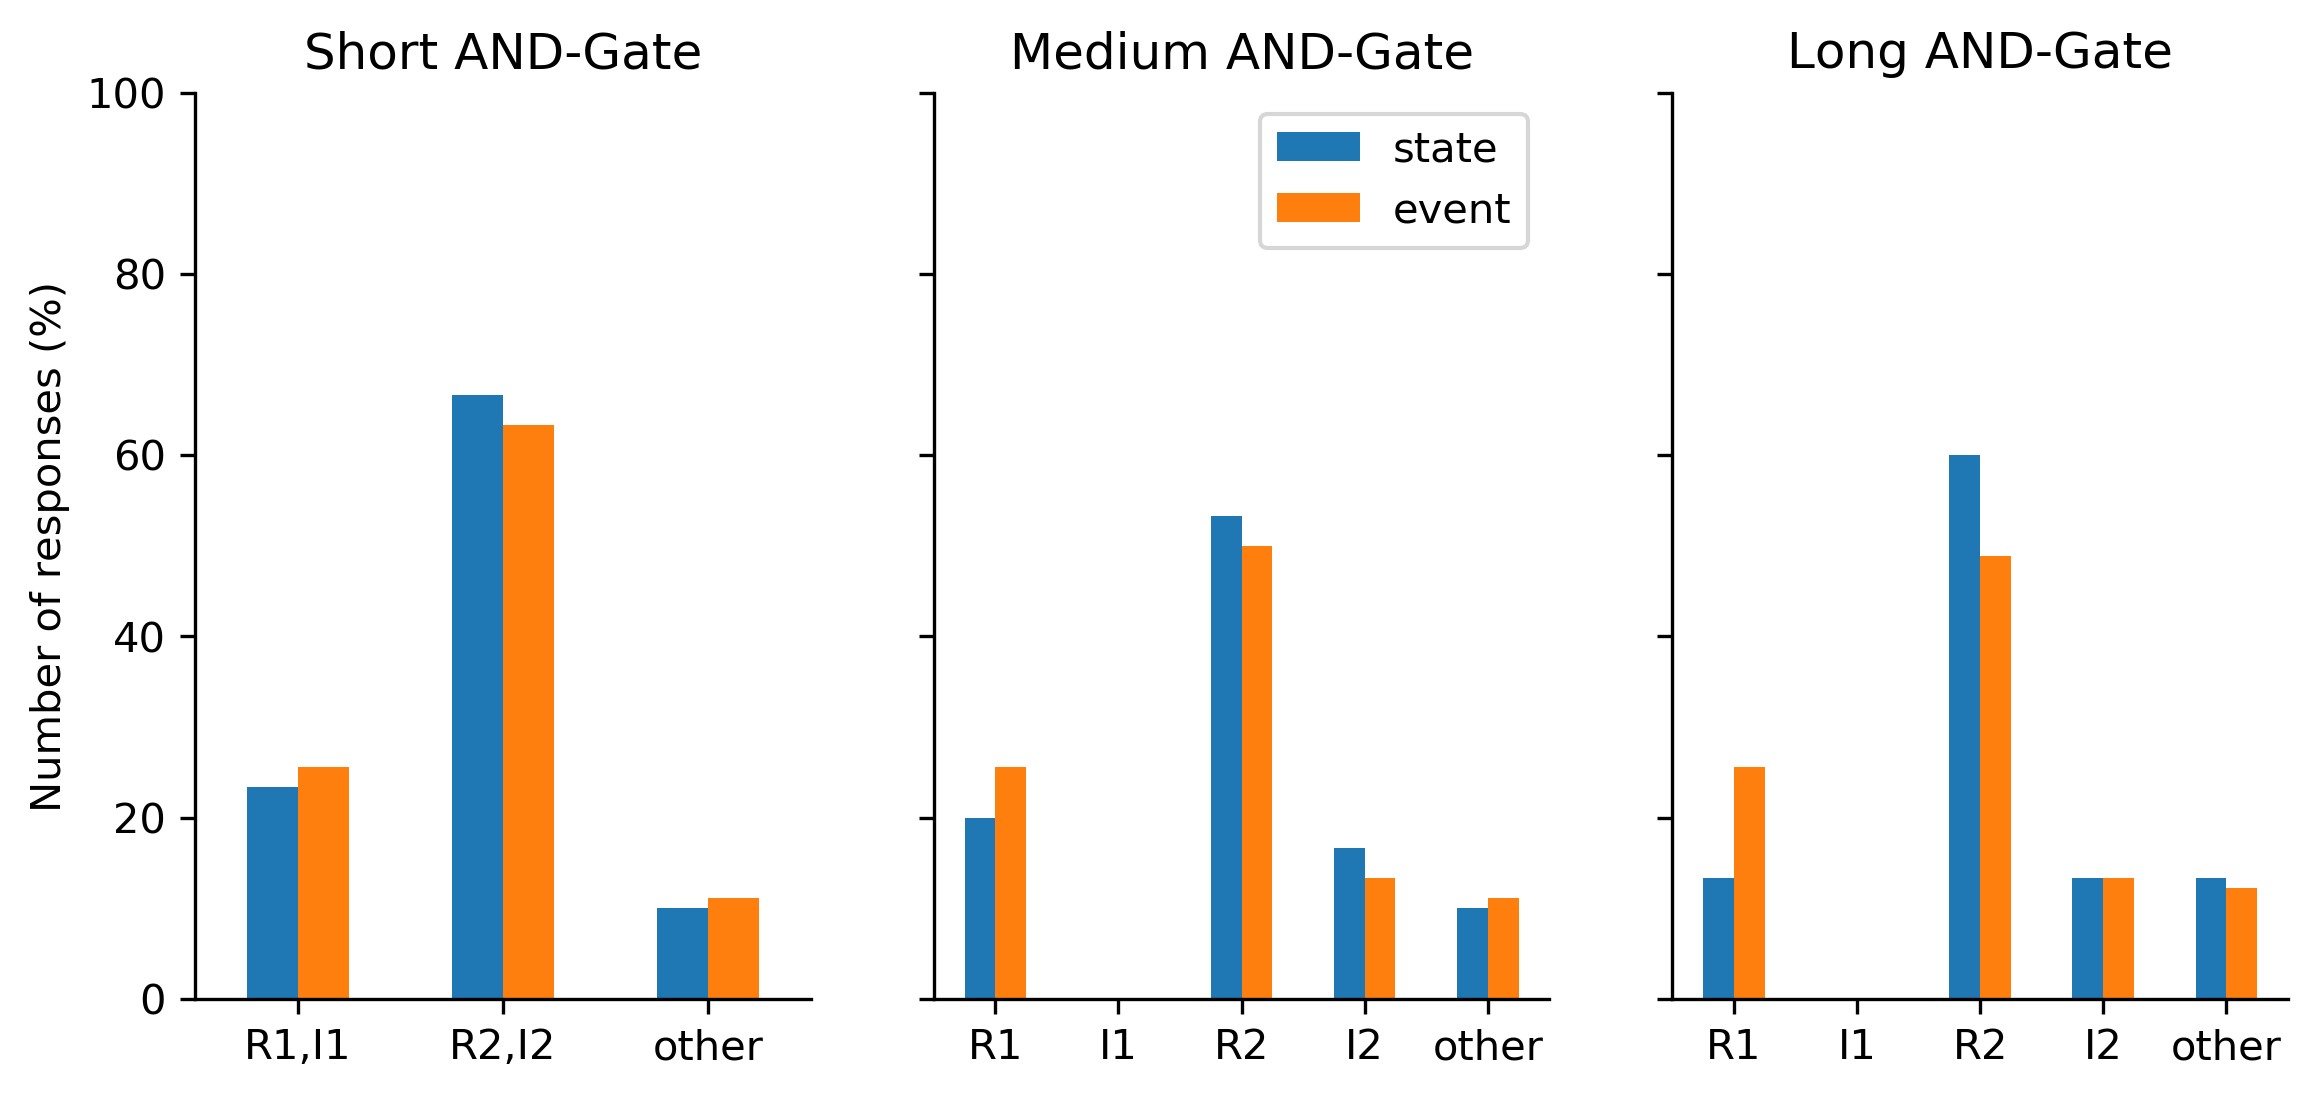
\includegraphics[width=8cm]{results_E1}
\end{center}
\caption{Comparison of the results for different length of activation in AND-Gates. Short: 1 activated detector in each branch. Medium: 3 activated detectors in each branch. Long: 6 activated detectors in each branch. ``State'' responses correspond to the networks where one branch was already activated before participants run the animation. ``Event'' responses correspond to the networks where no detectors were activated before and include results for 2s, 4s and 6s delays between I1 and R2. BUT SEE WARNING ABOVE.} 
\label{fig:2}
\end{figure}

\subsection{Experiment 2}

In the previous experiment we have seen that people generally chose R2 (identical to I2 in the short sequences) as the main the cause of the activation of the GCM. These results make sense since R2 and I2 are linked by a continuous sequence of changes. But this set up, where the first element of a chain ``waits'' for the occurrence of the last event of another chain before it can initiate a second sequence, is probably not the most common scenario in real life. For instance it might take more time for one causal process to end so that the causal process that has occurred first is not necessarily the one that ends first. In Experiment 2 we therefore wanted to break the temporal continuity between the root changes and the immediate changes of Experiment 1 such that the continuous sequence of changes be sometimes between R1 and I2 or R2 and I2. We predicted that when there is a continuous sequence of changes between R1 and I2, people would preferably choose R1 as the main cause.

\textbf{Participants}. The experiment was hosted by Google App Engine and 98 participants were recruited via Amazon Mechanical Turk. There were 40 females (average age: 40.4), 57 males (average age: 37.6) and 1 declared ``other''. All the participants were english speakers except for 2 participants.

\textbf{Method}. In Experiment 2 each participant was presented 7 different networks. One stimulus was a chain and all the other six stimuli were AND-Gates. Like in Experiment 1 we tested for the dimension ``Event'' \textit{vs} ``State''. Same as before in condition ``Event'' none of the detectors was initially active and in condition ``State'' one of the two branches was containing detectors that were already active before the animation started. However this time, within the condition ``Event'',  we also tested for the extra dimension ``R1 cont'' \textit{vs} ``R2 cont''.  In condition ``R1 cont'' (represented in Fig.\ref{fig:3}) the activation is such that there is a continuous sequence of changes going from R1 to I2 leading to the activation of G. In condition ``R2 cont'' (not represented here) this is R2 that was continously connected to I2 leading to the activation of G. For the AND-Gates the delay between I1 and I2 in condition ``Event'' was maintained at 11 nodes (i.e.1100 ms) for almost all the networks. There was only one network for which the delay was set at 8 nodes (800ms).

As in Experiment 1 participants were first presented the network in its initial state and were asked to click the ``Run'' button to observe an activation sequence over the network. Participants waited 5000ms to see a first change of state occurring in a detector. Activation delay between any two successive square activations was set on 100ms as well. All the stimuli were presented in a random order and participants were assigned to either group "Left" or "Right" as in Experiment 1, and each AND-Gate was randomly presented with the curved chain (see Fig.\ref{fig:3})) at the top or at the bottom.

\begin{figure}[ht]
\begin{center}
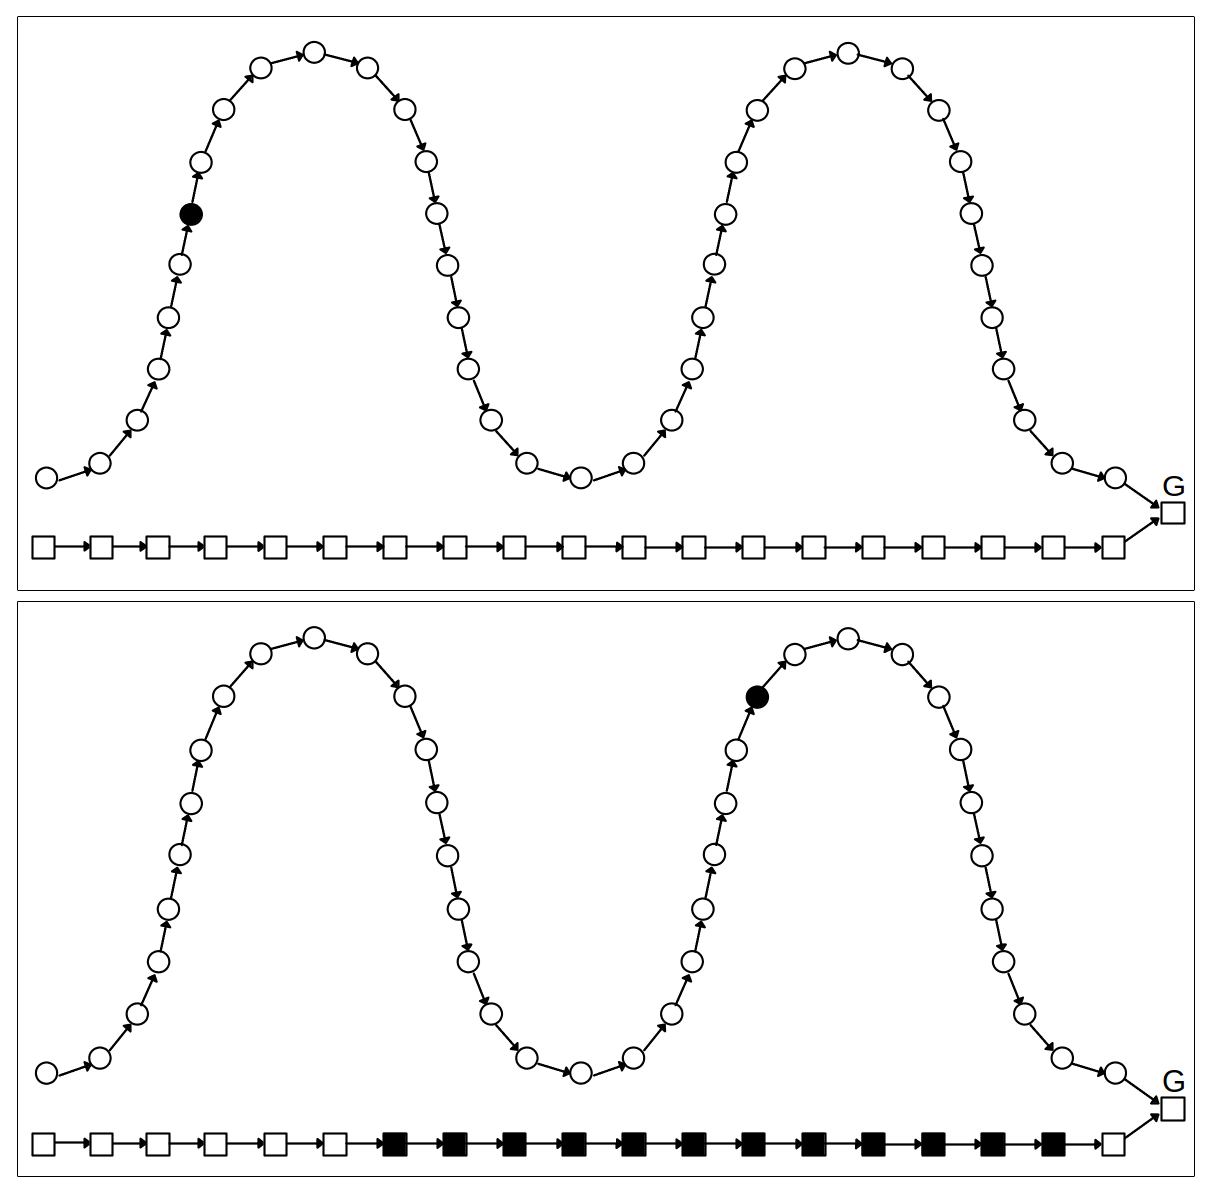
\includegraphics[width=8cm]{stim_E2a}
\end{center}
\caption{An example of an activation spreading over a network of Experiment 2. Here a continuous sequence of changes links R1 and I2 -- in other words this is the sequence of activations initiated by the chronologically first root change (curved branch) that eventually leads to the activation of the last immediate change and therefore G.} 
\label{fig:3}
\end{figure}


\textbf{Results}. First we observed no significant effect (statistics?) of neither the orientation of the networks (left \textit{vs} right) nor the location of the curved chain (top \textit{vs} bottom). On average participants took 8 min to complete the experiment and overall 91\% of the time participants run an animation only once. Second the reversed response pattern for R1 and R2 between ``R1 cont'', ``R2 cont'' and ``State'' stimuli type shown in (Fig.\ref{fig:4}) confirms our hypothesis: when this is the first root change R1 that initiates a continuous sequence of changes until the activation of G, R1 is considered the cause of the activation of G about two times more than R2 (31\% against 15\%) while this is the opposite when this is the second root change that initiates a continuous sequence of changes (18\% against 29\%). Coherently, for ``State'' condition (when this is R2 that initiates the continuous sequence of changes) participants prefer R2 over R1 in a very large extent (47\% against 5\%). As expected the type of network had however no effect on the responses for I1 nor I2 and the percentages of responses for I2 and the root change that initiates the continuous sequence for the Event network (31\% and 34\% for respectively the ``R1 cont'' and ``R2 cont'' networks) were approximately the same.

\begin{figure}[H]
\begin{center}
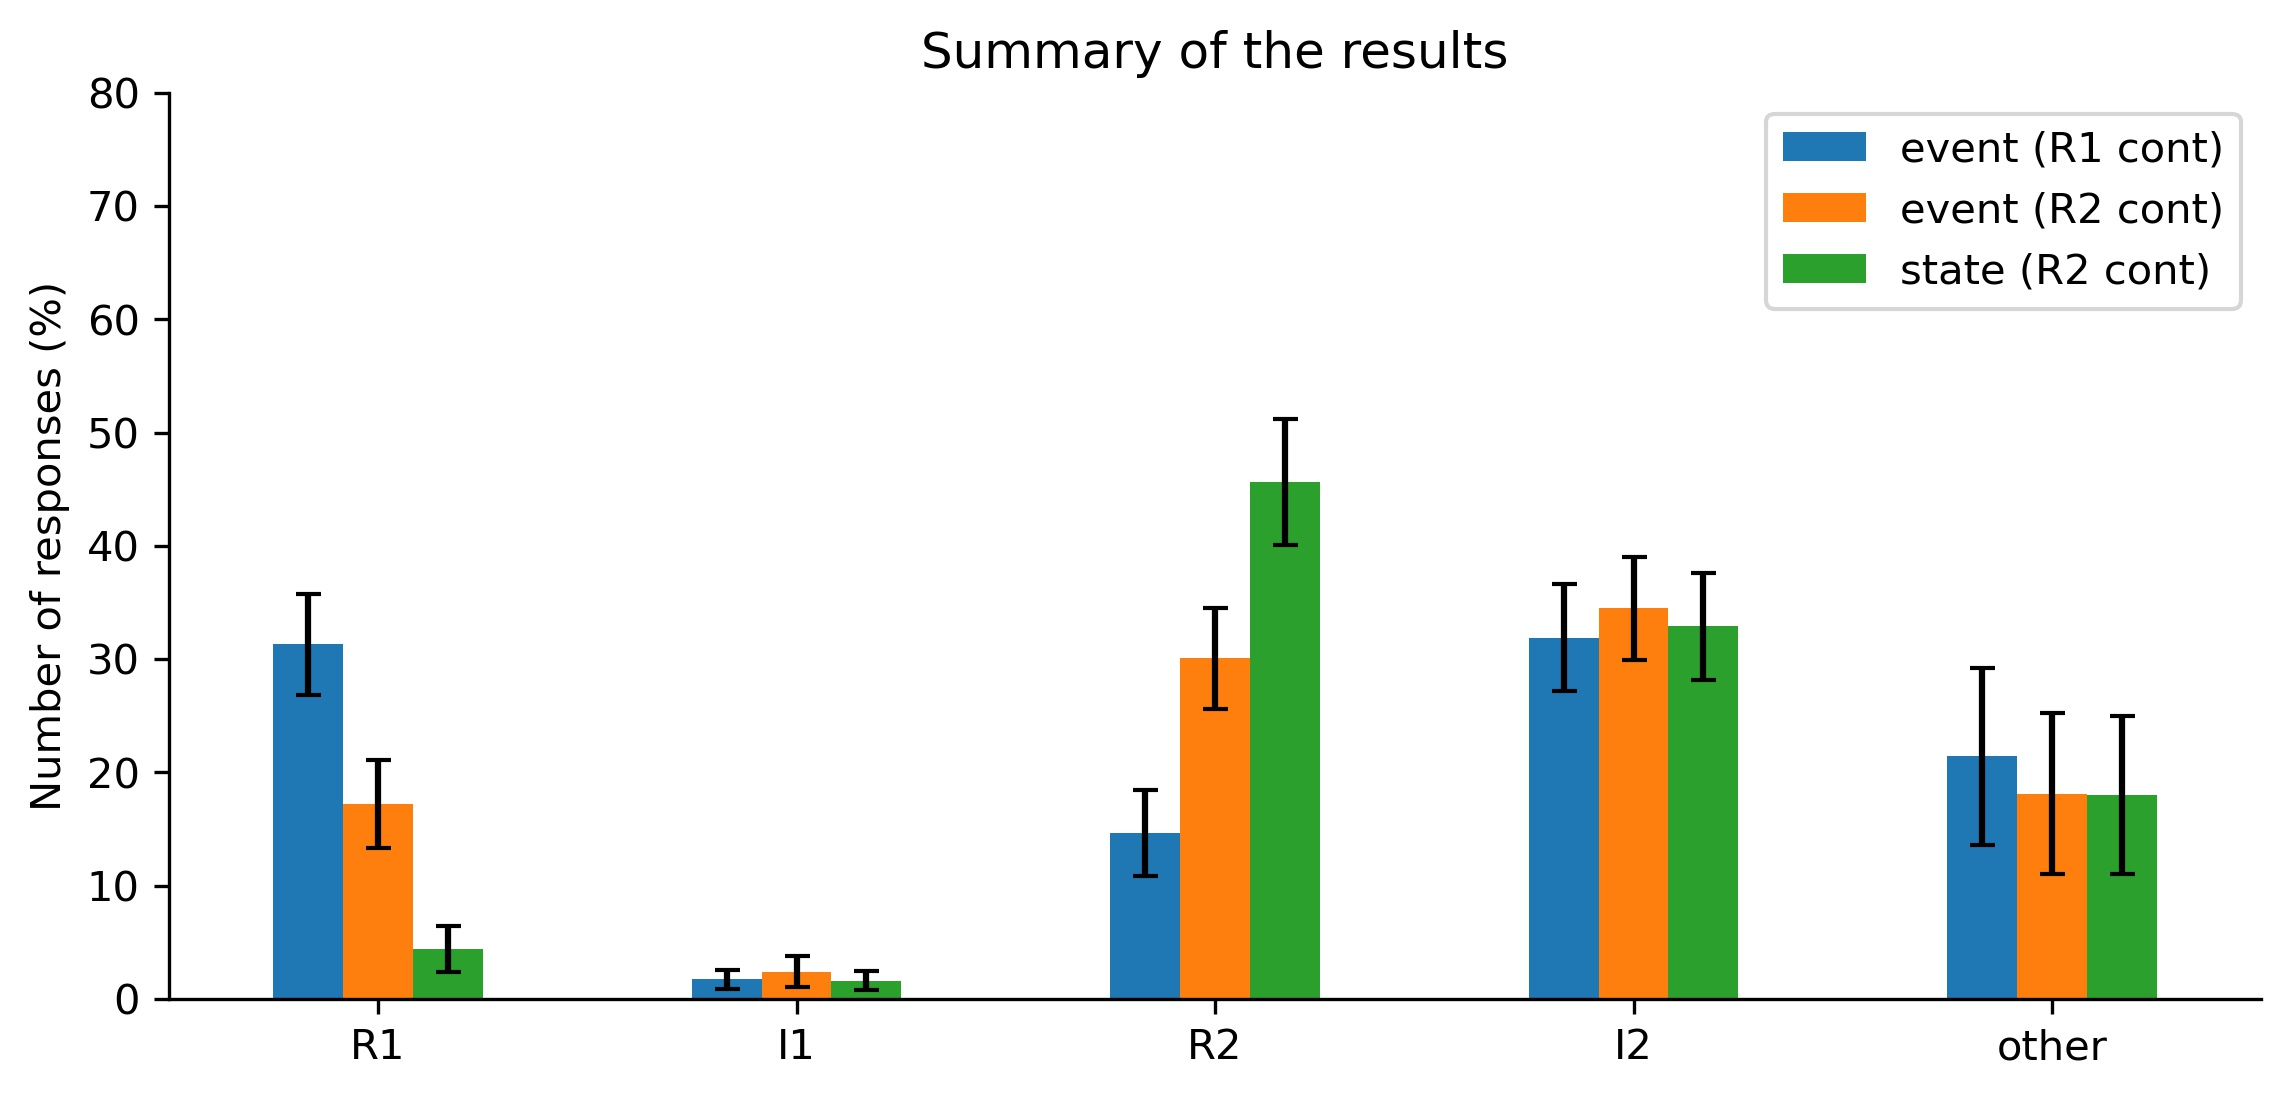
\includegraphics[width=8cm]{results_E2}
\end{center}
\caption{Results for AND-Gates where the continuous sequence of changes is either between R1 and I2 or between R2 and I2. ``Event (R1 cont)'': responses for the networks where no detectors were already active before the participant runs the animation and where the continuous sequence of changes is between R1 and I2. ``Event (R2 cont)'': responses for the networks where no detectors were already active and where the continuous sequence is between R2 and I2. ``State (R2cont)'': responses for networks where one branch was already activated before the participant runs the animation and where the continuous sequence of activation is necessarily initiated by R2.} 
\label{fig:4}
\end{figure}

\newpage
\section{General discussion}

Outline:

\textbf{I}. Summary and implications of the results

\textbf{II}. To say why these results cannot really be explained by the current theories of causation and why our theory can better account for them. I don't know if I should talk more about CF and PP accounts than I do in introduction, like saying something like that is probably not useful:

[\textit{According to the CF account, the general idea is that an event A is said to be a cause of a distinct event B if the occurrence of A makes a difference in the occurrence of B. More precisely A is a cause of B if and only if A and B are true, and A hadn't occurred B wouldn't have occurred. This interpretation calls upon counterfactual scenario or possible worlds where the presumed cause of the effect is removed from the system while all other relevant factors are kept as unchanged as possible compared to the actual world. According to us the main problem of this interpretation is that its best models explicitely rejects the idea of grounding causation on temporal information.
According to the PP account, an event A causes B when there is a physical connection between them. In one of its latest and probably most convincing formulation, this theory distinguishes two things : causal process and causal interaction (i.e. causation). A causal process is a physical process involving an object which conserves a certain quantity, like mass-energy, accross space and time. A causal interaction or causation is an exchange of that conserved quantity. However the theory goes sometimes against some of our best causal intuitions and to makes implicitely use of the CF analysis to explain our judgements: if I hold the head of my ennemy under water and make him die, I'm not genuinely the cause of his death; rather I'm actually preventing the possibility of a genuine causation which is breathing oxygen in order to live.}]

Or if I do have to explicit both theories I should insist on what the predictions of both theories are for our experiments and why they cannot explain people's intuition (the role of time).

\textbf{III}. To insist, maybe, on the work of Glymour where our project in part originated: explaining his caveat about treating events as pure propositions. To explain how our experiments extend this idea and insist more on the role of changes in continuous time. Maybe we should present some insights about how we could formalize further the model? How we could use formal tools like Graphical models?

\textbf{IV}. To present further experiments that would be interesting to make (with loops, cases of prevention, etc.)


\bibliographystyle{apacite}

\setlength{\bibleftmargin}{.125in}
\setlength{\bibindent}{-\bibleftmargin}

\bibliography{CogSci_Template}


\end{document}
